\section{Introduction}\label{sec:introduction}

For \(E\subset\R^d\), its Euclidean distance set is
\[
 \Delta(E)=\{|x-y|:x,y\in E\}.
\]
The Falconer distance conjecture asks whether a compact set of Hausdorff
dimension greater than half the ambient dimension must determine a set
of distances of positive length. We prove this assertion.

\begin{theorem}\label{thm:main}
Let \(d\ge2\) be an integer and let \(E\subset\R^d\) be compact. If
\(\dim_H E>d/2\), then
\[
 \cL^1(\Delta(E))>0.
\]
\end{theorem}

Theorem~\ref{thm:main} imposes no regularity beyond the strict Hausdorff
dimension assumption. In particular, it does not require equality of
Hausdorff and packing dimensions, an Ahlfors regular measure, product
structure, or Fourier decay. The assertion concerns positive Lebesgue
measure; a distance set of Hausdorff dimension one alone would not
suffice. The strict threshold is retained, and no endpoint assertion is made.

\subsection{History and scope}

The problem originates in Falconer's work~\cite{Falconer1985}, which
established the sufficient threshold \((d+1)/2\). His lattice-type examples
at dimension \(d/2\) explain the strict inequality in the positive-measure
formulation. Mattila's spherical-average criterion~\cite{Mattila1987}
made Fourier \(L^2\) estimates a central approach to the problem.
Bourgain connected improvements in dimensions two and three to Fourier
restriction phenomena on spheres~\cite{Bourgain1994}.
Among the subsequent milestones were Wolff's planar threshold
\(4/3\)~\cite{Wolff1999} and Erdo\u{g}an's threshold
\(d/2+1/3\) for \(d\ge3\)~\cite[Theorem~2]{Erdogan2005};
these positive-measure conclusions require strict dimension inequalities.
For the parallel finite point-set problem in \(\R^d\), \(d\ge3\), see the
distinct-distances theorem in~\cite[Theorem~1.1]{OpenAIDistinctDistances2026}.

Weighted restriction and decoupling led to further improvements.
Du, Guth, Ou, Wang, Wilson and Zhang obtained the threshold \(9/5\)
in dimension three and improvements in higher dimensions
\cite[Theorem~1.2]{DGOWWZ2021}. Du and Zhang obtained the threshold
\(d/2+1/4+1/(8d-4)\), improving the preceding bounds for \(d\ge4\)
\cite[Theorem~2.6]{DZ2019}.
The arguments draw on refined restriction estimates and on the
decoupling theory of Bourgain and Demeter~\cite{BD2015}.
For a pin \(y\), write
\(\Delta_y(E)=\{|x-y|:x\in E\}\).
Liu's \(L^2\) identity connects pinned distance measures with spherical
extension estimates and transfers spherical-average bounds to pinned
conclusions~\cite[Theorems~1.4 and~1.9]{Liu2019}.
The two preceding restriction advances also give
\(\cL^1(\Delta_y(E))>0\) for some \(y\in E\) under the corresponding
strict dimension inequalities; see \cite[Corollary~1.11]{DGOWWZ2021}
and \cite[Theorem~2.7]{DZ2019}.
For compact \(E\subset\R^2\) with \(\dim_HE>5/4\),
Guth, Iosevich, Ou and Wang proved the same pinned conclusion
\cite[Theorem~1.2]{GIOW2020}.
Their argument combines radial-projection control of discarded wave
packets with refined decoupling for the retained part.
Du, Iosevich, Ou, Wang and Zhang obtained the analogous pinned conclusion
in even dimensions \(d\ge4\) when
\(\dim_HE>d/2+1/4\)~\cite[Theorem~1.2]{DIOWZ2021}.
For compact \(E\subset\R^d\), \(d\ge3\), Du, Ou, Ren and Zhang
obtained the same existential pinned conclusion when
\[
 \dim_HE>\frac d2+\frac14-\frac1{8d+4}
\]
\cite[Theorem~1.2]{DORZ2024}.

At the critical dimension, Shmerkin and Wang proved that
\(\dim_H\Delta(E)=1\) for Borel
\(E\subset\R^d\), \(d\ge2\), whose Hausdorff and packing dimensions
both equal \(d/2\)~\cite[Theorem~1.4]{SW2025}.

For Borel \(E,F\subset\R^2\), Liu proved that
\(\dim_HE>1\), \(\dim_HE+\dim_HF>2\), and
\(\dim_HF=\dim_PF\) imply
\(\cL^1(\Delta_y(E))>0\) for some \(y\in F\)
\cite[Theorem~1.1]{Liu2026}.
Here \(\dim_P\) denotes packing dimension. Taking \(F=E\)
gives the conjectured planar conclusion for sets with equal
Hausdorff and packing dimensions greater than one.
The regularity of the pin set is a hypothesis of this result, not a
consequence of its Hausdorff dimension. Borges, Ou and Pasquariello
study positive measure for pinned \(k\)-star distance sets and admissible
distance-graph configurations~\cite[Theorem~A and Corollary~1.11]{BOP2026}.
Their \(k=1\) threshold lies above \(d/2\); they record the sharper earlier
one-edge bounds in~\cite[Remark~1.2]{BOP2026}. These results do not give
Theorem~\ref{thm:main}. The result here is unpinned; no corresponding
claim about a single pin is asserted at the threshold \(d/2\).

\subsection{Methodological antecedents}

The multiscale analysis of irregular measures has important precedents.
Keleti and Shmerkin decompose measures into dyadically regular pieces,
control bad projections across scale intervals, and optimize variations
of Lipschitz profiles in their work on the dimensions of planar distance
sets~\cite[Corollary~3.5, Section~3.2 and Section~5]{KS2019}.
These are antecedents for the regular classes, scale-dependent tests and
profile accounting used below. Their estimates concern Hausdorff dimension.
Their optimization controls a sum of interval drops;
Section~\ref{ledger:section} uses a potential built from two separated
depths to pay the present recursion's costs.
Shmerkin and Wang later combined scale profiles with radial projection
estimates and slicing~\cite[Sections~5.5 and~6.1--6.3]{SW2025}.

Our angular preparation is related to the multiscale incidence approach
of Orponen and Shmerkin~\cite[Section~1.5]{OS2023}, the radial thin-tube
bootstrap of Orponen, Shmerkin and Wang~\cite[Section~1.3]{OSW2024},
and the higher-dimensional radial and plate-concentration methods
of Ren~\cite{Ren2023} and Du, Ou, Ren and Zhang~\cite{DORZ2024}.
The retained incidence input is the theorem of Orponen and Shmerkin
\cite[Theorem~1.3 and Remark~1.4]{OS2023}, in the tube formulation of
\cite[Definitions~2.5--2.6 and Theorem~2.7]{OSW2024}.
The auxiliary radial estimate is proved here by Orponen's finite-energy
method~\cite[Section~3 and the proof of Theorem~1.13]{Orponen2019}.
It is applied only in a dimension where its energy hypotheses hold.

Auxiliary projections used to prepare radial information, while keeping
the final distance map in the original space, also occur in
\cite[Sections~2--3]{DIOWZ2021}.
The separation between approximation of a distance measure and Fourier
control of its retained part has a precedent in
\cite[Propositions~2.1--2.2]{GIOW2020}.
Liu's regular-pin theorem uses a multiscale good--bad decomposition and
weighted extension estimates~\cite[Section~1.1]{Liu2026}.
These comparisons describe relationships between methods, not additional
theorem inputs. The present proof supplies its angular tests, oscillatory
graph reductions, two-depth potential and monotone shell reconstruction;
it does not invoke a decoupling theorem or any earlier distance theorem
at an improved threshold.

\subsection{The two main issues}

Put \(S=d/2\). An immediate obstacle in higher dimensions is that
radial projections of a separated \(s\)-dimensional source cannot acquire
dimension greater than \(s\). Thus, when \(S<s<d-1\), one cannot assume that
these projections have densities relative to surface measure on
\(S^{d-1}\). The first part of the proof constructs instead the cap bounds
that the Fourier argument actually needs.

After restriction to two separated Frostman measures, we form decreasing
sets of admissible pairs, denoted by \(\Gamma_N\). Their intersection has
positive product mass. At each scale \(2^{-N}\), a further exceptional set
of pairs of power-small mass can be deleted so that every remaining
directional fiber has a cap bound of exponent \(S\), with an arbitrarily
small power loss. Here a directional fiber is the opposite measure,
restricted by the pair condition at a fixed endpoint and then pushed to
the sphere by the radial map; it is not normalized separately.
Integer exponents
come from supercritical radial integrability after projection to a smaller
space. In odd dimensions, a thin-tube improvement supplies the additional
half dimension. Its linear gain is proved by slicing to the plane; the
integer endpoint requires a separate transverse-triple argument.

The auxiliary projections concern directions and incidences only.
Every distance and every oscillatory distance phase in the rest of the
proof is taken in the original space \(\R^d\).

The second issue is to exploit these fractal angular laws in a distance
estimate. A cap test controls parallel tubes, whereas a scalar projection
test involves belts on the sphere. The required belt estimate follows
from a Fourier calculation: the annular power is \(B^{d-2S}\), which is
exactly one at \(S=d/2\). This gives the angular tests used by the
recursive reductions.

\subsection{From profiles to a distance measure}

At a fixed dyadic frequency \(R=2^N\), decompose each Frostman measure into
almost uniform dyadic classes. If a class has mass profile \(m\), write
\[
 A_n=m(n/N)-S n/N.
\]
Thus its occupied depth-\(n\) cells have mass approximately
\(R^{-m(n/N)}\), up to the controlled regularization loss.
The excess profile \(A\) records decay beyond the critical exponent \(S\).
The two recursive quantities are a count of pairs with nearly
equal distances, denoted by \(\mathsf D\), and a product of spherical
Fourier energies with independent angular variables, denoted by
\(\mathsf H\). The high-frequency part of \(\mathsf D\) is split into
distance-frequency shells. Stationary phase first produces the square of an angular inner product
\(\mathsf H_F\), which Cauchy--Schwarz bounds by \(\mathsf H\).
The graph estimate then uses the parallel tests to advance to finer
cells. Other reductions return to positive distance counts or shorten
the interval of scales. The definitions and the conversions appear in
Sections~\ref{osc:section}--\ref{rec:section}.

An angular state carries tests selected on an interval containing the one
currently being estimated. Each test is retained until the recursion
reaches its associated depth. A potential formed from two values of \(A_n\)
at sufficiently separated depths is evaluated on the current interval.
It pays the positive step costs and closes the recursion.

For two profiles, let \(c\) be the last depth at which either excess
profile is at most a fixed small level \(\beta>0\). The graph estimate
passes the independent angular energy to cells at depth \(c\).
Cauchy--Schwarz in the radial variable bounds this by the geometric
mean of two single-profile states, so the recursive bound applies.
Each potential is at least \(2\beta-O_d(1/N)\), while the entry cost
is at most \(\beta\) up to the regularization loss. The profile
increments cancel, leaving a strictly decaying Fourier shell bound
once the losses are chosen sufficiently small; see
Lemma~\ref{asm:entry} and Proposition~\ref{asm:shell-decay}.

The coarse pair restrictions \(\Gamma_N\) need not converge at a
quantitative rate. We therefore use the following form of the scalar
shell principle. If positive measures \(\alpha_N\) decrease to
\(\alpha_\infty\), if
\[
 \|\alpha_N-\tau_N\|_{\TV}\lesssim 2^{-\eta N},
 \qquad
 \int_{2^{N-1}\le |r|\le2^{N+1}}
       |\widehat{\tau_N}(r)|^2\,\dd r\lesssim 2^{-\gamma N},
\]
and if \(\eta,\gamma>0\), then \(\alpha_\infty\) is absolutely continuous.
The proof uses summable positive increments
\(\alpha_n-\alpha_{n+1}\) and telescoping smooth Fourier cutoffs;
it is given in Lemma~\ref{asm:monotone-shell}.
Our limiting measure is nonzero and carried by \(\Delta(E)\), which proves
Theorem~\ref{thm:main} in Section~\ref{sec:assembly}.

The components that may be useful separately are the thin-tube upgrade
(Proposition~\ref{prep:thin-upgrade}), the critical fractal angular
Fourier estimate (Lemma~\ref{test:half-dimensional-fourier}), the graph
estimate with independent angular variables
(Proposition~\ref{graph:estimate}), and the monotone-measure shell
principle (Lemma~\ref{asm:monotone-shell}).

Figure~\ref{fig:proof-map} summarizes the roles of the auxiliary and
original spaces.
\begin{figure}[t]
 \centering
 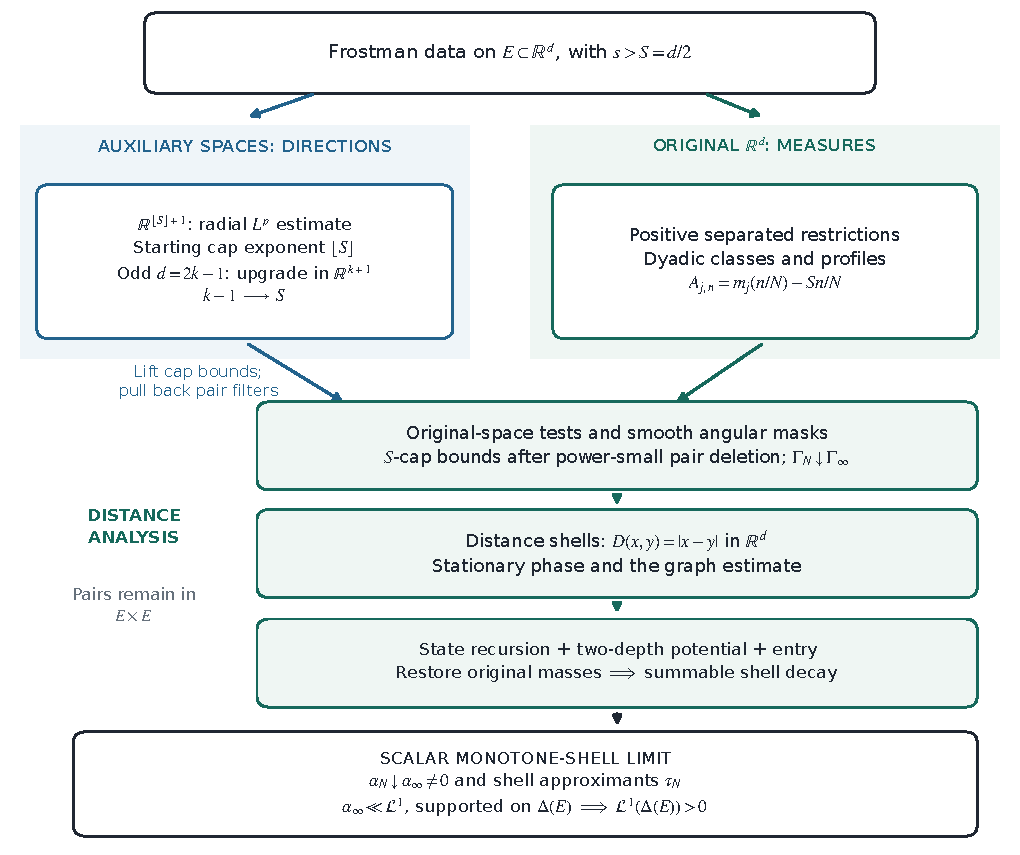
\includegraphics[width=\textwidth]{figures/proof-map.pdf}
 \caption{The main construction.
 Auxiliary projections prepare directional bounds and pair filters;
 the cap bounds hold after an additional power-small pair deletion.
 These data return to the original space, where the argument uses the
 Euclidean distance of the original pairs. The decreasing filters and
 shell-dependent approximants meet in the final scalar monotone-shell argument.}
 \label{fig:proof-map}
\end{figure}
